
%%%%%%%%%%%%%%%%%%%%%
% A

\appendix
\renewcommand{\thesection}{\arabic{section}}

\chapter{Gannt Diagram}
\label{appendix:A}

\begin{figure}[H]
  \centering
    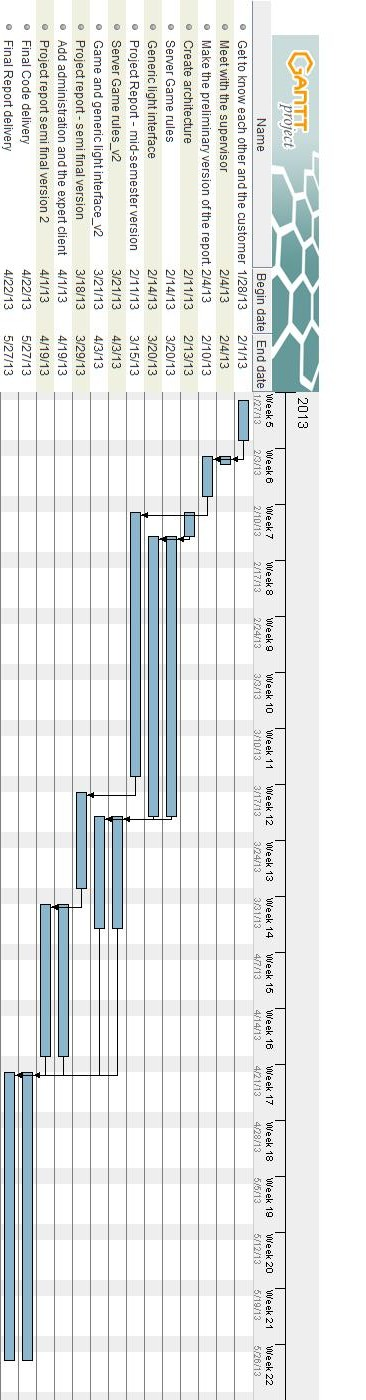
\includegraphics[height=20cm]{img/ganttv3v2.jpg}
  \caption{ 'Gannt diagram'} 
  \label{fig:ganntDiagram}
\end{figure}





%%%%%%%%%%%%%%%%%%%%%
% B

\chapter{Don't Panic board game rules}
\label{appendix:B}
%
\emph{These are the rules of the physical board game, supplied by the customer.}
%
%
\section*{Description of the game}
Don’t Panic is a cooperative game. You start the game as member of a “panic control team”. During your day different potential panicking events will take place and you and your team will have to work together to calm people down and prevent the day from becoming the worst panic event humanity has ever seen. You and your teammates will assume a unique role within the team, with special abilities that will improve your team’s chances, if applied wisely.\\
\\
The aim of the game is to calm the situation down. In the game you can calm people by
\begin{itemize}
	\item opening/blocking paths to help people to get off from frightening situations
	\item talking with them while other solutions are applied
	\item sharing information about how to manage the crisis
	\item moving people from one sector to another. But be careful! You only have a limited time to contain panic.
\end{itemize}
Every 5 minute the “panic level” will increase as a new “panic wave” arrives! If you and your team are unable to keep the panic contained and apply the necessary strategies to calm the people down in time, your city will become a mess and you and your team will lose the game.\\
%
%
\subsection*{A game turn}
The play proceeds clockwise around the table with each player taking turns (in order) until the game ends. For each turn, the current player MUST
\begin{itemize}
	\item take 	4 ACTIONS
	\item draw 	2 INFORMATION CARDS to add to his hand	
	\item draw 	2 EVENT CARDS and perform the corresponding actions on the board
\end{itemize}
%
%
\subsection*{Actions}
A player gets 4 actions to spend on her turn. A given action may be performed more than once during a turn, so long as 1 action is spent for each instance. Each player’s role will grant them special abilities that are unique to that player. Players may also pass if they have nothing else to do. Unused actions CANNOT be saved from turn to turn.\\
\\
In each action the player can
\begin{itemize}
	\item calm 5 people in a sector down
	\item move 5 people from one sector to another
	\item move through a maximum of 3 nodes
	\item create a barrier (is done with the help of another player)	
	\item remove a barrier (is done with the help of another player) 	
	\item decide to spend all his actions in order to create an information center
\end{itemize}
%
%
\subsection*{Components}
1 BOARD represents a real or virtual city. The board is divided into sectors and presents paths and key points. If all the paths in a sector are secured (i.e. blocked) the sector is secured (that is the panic will not augment in the sector at the next wave). However, only a non-secured path can let people pass from one sector to another.\\
\\
8 PAWNS represent the players. The color of the pawn is linked to the draw role card. The pawn moves towards the sectors following key points. The player can act only on the sectors communicating with the key point.\\
\\
1 TIMER calculates the next panic wave. When the timer rings each already panicked sector will be incremented by 5 panicked people (PL). In the non-panicked sectors nothing will happen. During the game panic waves happen initially every 10 minutes, then every 7 minutes and then every 5 minutes.\\
\\
94 PLAYER CARDS :
\begin{itemize}
	\item 6 ROLE CARDS. Each player assumes a specific role in the game which can do particular actions at low cost. The roles are detailed below.
	\item 48 EVENT CARDS. Event cards are, together with the Timer, the source of panic. Each round the player has to draw 2 event cards and apply their effects.
	\item 40 INFORMATION CARDS. Information cards diffuse information which is useful to manage panic. Playing an information card is at 0 cost (i.e. it is an additional action the player can take). Only one card per round can be played and only by the current player. 
\end{itemize}
%
INFORMATION CARDS can be exchanged, but only if the two players are on the same key point. Each round the player has to draw 2 information cards but he can use them only from the next round. Take care! The number of information cards is limited! Once used, they cannot be put back into play.\\
\\
5 INFORMATION CENTERS help lowering the panic. Once an information center has been constructed, the effects of the (draw)?? event cards on the adjacent zone are cut by half. However, creating an information center is a highly costly action. To construct an information center a player needs to use all his actions for this round. A maximum of 5 information centers can be created on a board.\\
\\
DISPLAYS WITH PANIC NUMBERS. Each sector of the game is equipped with a display to indicate the panic level (PL) in the sector. Chain Reactions: Once the panic number reaches quota 50 (that is 50 people panicked in the zone) the panic propagates to all nearby sectors (+5 panicked people). \\
\\
10 BARRIERS help to block the spreading of panic throughout the sectors. To make a zone safe, all the paths have to be blocked. However, people cannot pass through blocked sectors. To create a barrier TWO players have to be on the same key point at the same time. \\
%
%
\subsection*{Sharing Information}
Don’t Panic is a collaborative game! Players are encouraged to openly discuss strategies during the game and share information. An information card can be used only once in a turn but it does not cost any action. Information can be “transferred” from one player to another. To transfer an information card from one player to another, the players have to be on the same key point. Only one card can be transferred at a time. The player who has the role of the Coordinator can transfer a card even if he is not on the same key point. \\
\\
\subsection*{Roles}
Each player is assigned a certain role, and there are six different roles:\\
COORDINATOR : Can share information even if he is not on the same key point\\
CROWD MANAGER: Can calm down 10 people in each sector instead of 5\\
DRIVER: Can move 10 people from one sector to another\\
OPERATION EXPERT: Can create/remove a barrier alone\\
VOLUNTEER: Can support one of the players (apart from the coordinator) duplicating their last action\\
PASSER BY: Can pass 1 information card to a player in an adjacent sector\\
\\
\subsection*{Setting up the game}
\begin{enumerate}
	\item Place the board in the center of the table within easy reach of all the players. Put the displays on the board.
	\item Shuffle the Role cards and deal 1 to each player. Each player takes their corresponding colored pawn. Place the pawn on the big matching colored key point. If the main key point is already taken, choose the small matching colored key point. Put excess Role cards and pawns (if any) back into the box.
	\item Shuffle the INFORMATION CARD cards and deal them to the players face down. For a \\4 PLAYER GAME: 2 CARDS EACH.  \\3 PLAYER GAME: 3 CARDS EACH. \\2 PLAYER GAME: 4 CARDS EACH. \\Place the remaining INFORMATION CARDS face down on the board in the appropriate sector. 	
	\item Shuffle the EVENT CARDS and place them face down on the board in the 	appropriate sector.
	\item Put the initial panic on the board: Each player draws 1 card from the EVENT CARDS and performs the corresponding action.
	\item Turn the INFORMATION CARDS and communicate the possible actions you can perform.
	\item Start the timer.
	\item Play the game! 	
\end{enumerate}

N.B. For a more challenging game session, switch the points 6 and 7. \\
%
\subsection*{Defeat and victory!}
The game ends immediately in defeat for all players if all the map has a panic level higher than 50 panicked people. Players collectively win the game when the panic can no more spread because of the barriers, or if there is no panic on the board.

%%%%%%%%%%%%%%%%%%%%%
% C

\chapter{Updated Don't Panic game rules}
\label{appendix:C}
%
\emph{There were several changes in the rules of the board game to the electronic version. These changes have been acounted for in the updated rules.}
%
%
\section*{Description of the game}
Don’t Panic is a cooperative game. The players start the game as members of a “panic control team”. During the game different potential panicking events will take place and the team will have to work together to calm people down and prevent the day from becoming the worst panic event humanity has ever seen. The players will assume specific roles within the team, with special abilities.
\\
The aim of the game is to take charge of a city and keep the city from panicking. As a player you can calm down the people by:
\begin{itemize}
	\item using Information Cards given to the players. Which zones are affected depends on the specific Information Card.
	\item selecting the Zone you want to decrease panic in, and clicking the "Decrease panic"-button.
\end{itemize}
The timer in the game counts down to the next “panic wave”, where the panic levels of the Zones increase by a certain value. This value is set by the expert when setting up the game. Zones that have no panic are not affected by this. \\
%
%
\subsection*{Turns}
Each player takes turns playing the game, until the game ends. During their turns, the players receive 1 Information Card and 4 Action Points they can use in the game. Events also happen during turns. How often Events happen is decided by the Expert when the game is set up.
%
%
\subsection*{Actions}
Any action the player does during their turn may be performed more than once, as long as the player has enough action points. Players may also pass if they do not want to do any actions. Unused actions from one turn are not saved onto the next turn.\\
\\
The players can use their action points to:
\begin{itemize}
	\item decrease panic by 5 in a Zone, or 10 if the player is a Crowd Manager (costs 1 action point)
	\item move 5 people, or 10 if the player is a Driver, from one Zone to another. The Zones have to be adjacent (costs 1 action point)
	\item move to an adjacent Node (costs 1 action point)
	\item create a Roadblock on a node. This can only be done if there is another player on the same node, unless the player is an Operation Expert (costs 1 action point)	
	\item remove a Roadblock on a node. This can only be done if there is another player on the same node, unless the player is an Operation Expert (costs 1 action point)	
	\item create an Information Center on a node (costs 4 action points)
\end{itemize}
%
%
\subsection*{Components}
The map is divided into Zones which are separated by paths between the nodes. If all the nodes in a zone are secured (i.e. they have Roadblocks) the zone is blocked. This means that if the panic in a zone has reached 50, the panic will NOT spread to adjacent Zones, unlike unblocked Zones. However, the players can not move people between Zones if all their nodes have Roadblocks.\\
\\
The players are represented by “pawns”. Each pawn is represented by an icon, which tells the players which roles they are. The players can move their pawns on paths between the Nodes, and they can act only on the Node they're located on or the Zones adjacent to the Node.\\
The timer counts down to when the next panic wave arrives. When the timer reaches zero, the panic in all the already paniced Zones will increase. The amount of panic the Zones increase with is related to how many people are in that Zone. How much time the players have before the panic waves starts is set by the Expert.\\
\\
The players receive one information card at the start of each turn. The cards do not cost action posts to use, but there is a finite number of cards, so the players should be careful when using them. The total amount of Information Cards in the game is set by the Expert.
\\
The Information Center helps to lower the panic. Once an Information Center has been constructed in a Node, the effects of Events on Zones connected to the Node with the Information Center are cut by half. The maximum amount of Informations Centers allowed in the game is set by the Expert.\\
\\
Roadblocks help to block the spreading of panic throughout the Zones. All Nodes of a Zone have to be blocked for the Zone to be completely blocked. People cannot pass through blocked Zones.\\
\\
Each Zone in the game is equipped with a display to indicate both the panic level and number of people in the Zone. Once the panic reaches 50, the panic spreads to all nearby Zones, increasing their paic by 5. If a Zone is completely blocked, the panic will not spread. The amount of people in a Zone affect the increase in panic during a panic wave\\
%
\subsection*{Roles}
Each player is assigned a certain role, and there are three different roles:
\begin{itemize}
	\item Crowd Manager: Can calm down 10 people in a Zone instead of 5
	\item Driver: Can move 10 people from one Zone to another instead of 5
	\item Operation Expert: Can create/remove a Roadblock alone
\end{itemize}
%
\subsection*{Setting up the game}
\begin{enumerate}
	\item The Expert sets up the game by creating a template. The template holds all the information for the state of the game, such as Information Cards, Events, Roles of the players and initial panic in the Zones of the map.
	\item When the Expert is done, the Players start the game by choosing the correct template in their client, which starts the game.
\end{enumerate}
%
\subsection*{Defeat and victory!}
The game ends immediately in defeat for all players if all Zones on the map reach 50 panic. Players collectively win the game when there is no panic left on the board.

%%%%%%%%%%%%%%%%%%%%%
% D

\chapter{User manual}
\label{appendix:D}
%
This is a high level description of how to play Don't Panic! The game is started by accessing the game server through a web browser (if you are running a local server, use 127.0.0.1:8008). When starting the program, the user is given four choices:

\begin{figure}[H]
  \centering
    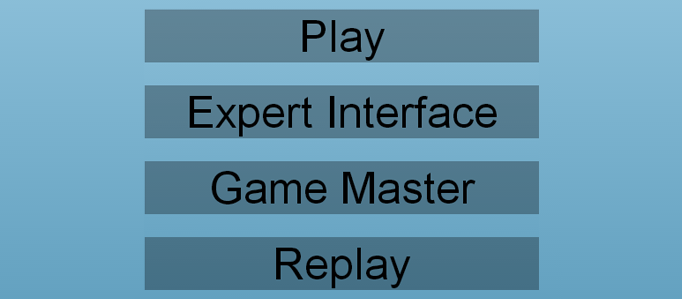
\includegraphics[width=1.0\textwidth]{img/choices.png}
  \caption{User Manual, 'The different choices for the user when starting the game'}
  \label{fig:choices}
\end{figure}

\section{Play}

When clicking the Play-button, a list of the available game-templates is shown:

\begin{figure}[H]
  \centering
    
\includegraphics[width=1.0\textwidth]{img/gamelist.png}
  \caption{User Manual, 'List of templates'}
  \label{fig:gamelist}
\end{figure}

\noindent After choosing a template, the program will start a new game with the given template as the initial state of the game. The users will now be able to play the game by moving their game pieces and pressing buttons.

\begin{figure}[H]
  \centering
    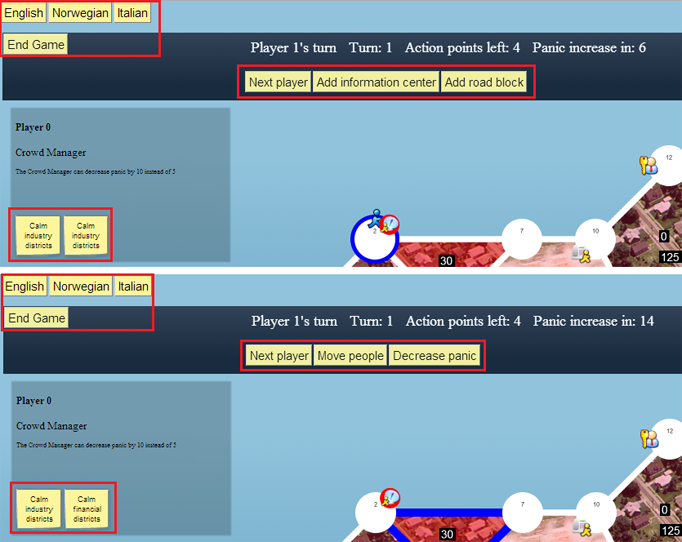
\includegraphics[width=1.0\textwidth]{img/buttonsbothred.png}
  \caption{User Manual, 'The different buttons in the game'}
  \label{fig:buttons}
\end{figure}

\noindent The available buttons depends on if a player has selected a zone or a node. As seen in the images above, the top screenshot shows the buttons available when selecting a node, while the bottom one shows the buttons available when selecting a zone. The buttons for adding and removing roadblocks, information center, moving people and decreasing panic are not available when neither a zone nor a node is selected.

\begin{itemize}
\item Buttons - 'English', 'Norwegian', 'Italian', chooses the language for the game (Italian has not been implemented).
\item Button - 'End Game', ends the current game.
\item Button - 'Next player', changes the turn.
\item Button - 'Move people', moves people from this zone to the next zone pressed.
\item Button - 'Decrease panic', decrease the panic in this zone.
\item Button - 'Add information center', add an information center in this node.
\item Button - 'Add road block', add a road block in this node.
\item Button - 'Remove road block', remove the road block in this node.
\item Button - 'Use information card', use one of your information cards.
\end{itemize}

\section{Expert interface}

The Expert Interface is used to set up game templates. All the information for a game, such as map, cards and players are set up in this interface, and stored on the database to be used when starting a game session.

\begin{figure}[H]
  \centering
    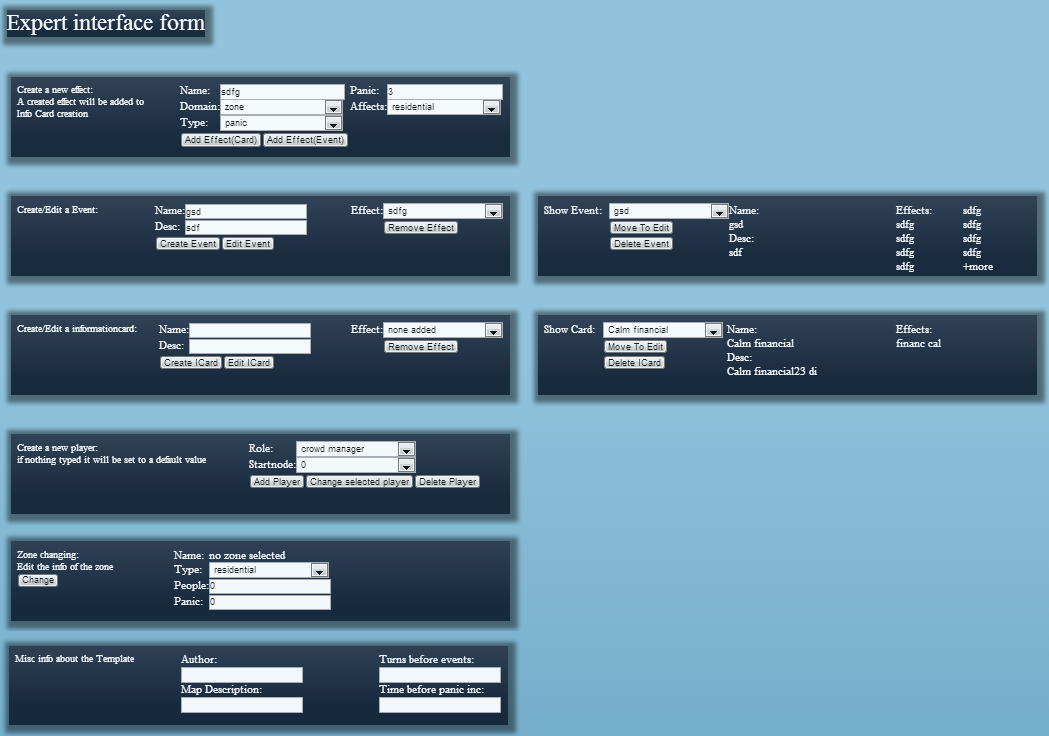
\includegraphics[width=1.0\textwidth]{img/ExpertInterfaceForms.png}
  \caption{User Manual, 'The Expert Interface forms used to set up the game'}
  \label{fig:expertinterface}
\end{figure}

\begin{itemize}
\item Create new effect: Type in the wanted name for the effect, change in panic, what domain the effect is for, what type of zone the effect affects and what type of effect it is. Then add the effect as a card- or event effect using the buttons.
\item Create/edit a event: Type in the wanted name for the event, add an effect, and write a description of the event. This description will be visible to the players in the game when the event happens. Use the buttons to create the new event, edit an event or remove the effect. The available events can be browsed by using 'Show Event'. To edit an event, it has to be selected in 'Show event', and then clicking 'Move To Edit'
\item Create/edit a information card: Type in the wanted name for the card, the wanted effect and a description of the card. The description is visible to the players. The available information cards can be browsed by using 'Show Card'. To edit an information card, it has to be selected in 'Show card', and then clicking 'Move To Edit'
\item Create a new player: Choose the wanted role and startnode of this player. Then click 'Add player'. Players can also be deleted by clicking 'Delete Player'.
\item Zone changing: Edits the information of the selected zone. The zone is selected by clicking on it in the canvas. You can edit the type of zone and the amout of people and panic.
\item Misc info about the template: Type in name of the author, a description of the map, the amount of turns before events should happen and the initial time before panic increases in the game.
\end{itemize}

\noindent In the bottom of the expert interface there is a canvas for drawing the map of the game.

\begin{figure}[H]
  \centering
    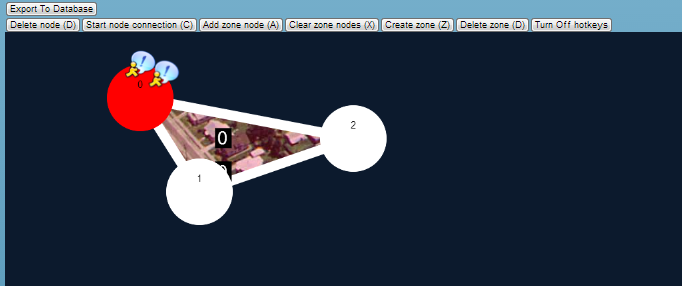
\includegraphics[width=1.0\textwidth]{img/expertinterfacecanvasmanual.png}
  \caption{User Manual, 'The Expert Interface canvas for creating a map'}
  \label{fig:expertinterfacecanvas}
\end{figure}

\noindent Left click in the canvas to create a new node. A node is red to indicate that it is selected. A node can be moved by dragging it with the mouse.
 
\begin{itemize}
\item Button - Delete node(D): Deletes the selected node from the map, D is the shortcut for this action on the keyboard.
\item Button - Start node connection(C): Starts a node connection from the selected node to the next, select another node to create a connection between them. A black line between the nodes represents the connection. A player can only move between nodes that are connected.
\item Button - Add zone node(A): Readies a node to be added to a zone (when creating a zone, you must first add them using this function). A node will turn blue to indicate that it has been marked as a zone-node.
\item Button - Create zone(Z): Select the nodes for the zone using Add zone node(A), then press this button. A zone will now have been created from the nodes selected.
\item Button - Clear zone nodes(X): Clears all the selected nodes that are a zone node. The blue zones will turn white to indicate that they have been cleared.
\item Button - Delete zone(D): Deletes the selected zone.
\item Button - Turn off hotkeys: Turns of the hotkey functionality. This is useful when typing in the form.
\end{itemize}

\section{Game Master}

A list of games in progress will be displayed when choosing Game Master from the main menu.

\begin{figure}[H]
  \centering
    
\includegraphics[width=1.0\textwidth]{img/gamemasterlist.png}
  \caption{User Manual, 'The list of games being played'}
  \label{fig:replaylist}
\end{figure}

\noindent Choose one of the available games to enter as a game master. The game master will now be able to watch the game being played in real-time, as well as interact with the game as he chooses, as if he was a player in the game. The game master can do actions regardless of whose turn it is.

\section{Replay}

The current replays are displayed when selecting 'Replay' from the main menu. A replay is a finished game that has been stored to the database. Chose one of them from the list, and the chosen replay will start.

\begin{figure}[H]
  \centering
    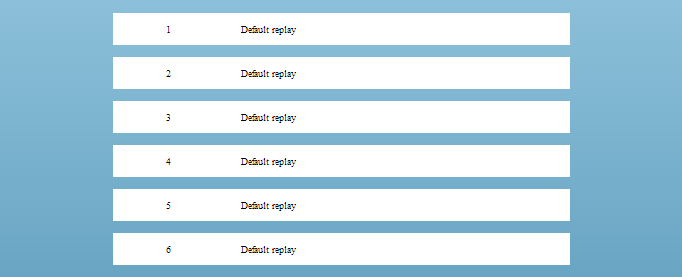
\includegraphics[width=1.0\textwidth]{img/replays.png}
  \caption{User Manual, 'The list of available replays'}
  \label{fig:replaylist}
\end{figure}

The replay view is identical to the game view, but the user can only use two buttons:

\begin{figure}[H]
  \centering
    
\includegraphics[width=1.0\textwidth]{img/replaybuttons.png}
  \caption{User Manual, 'Buttons used in replay view'}
  \label{fig:replaylist}
\end{figure}

\begin{itemize}
\item Button - Previous action: will display the previous game state of the replay.
\item Button - Next action: will display the next game state of the replay.
\end{itemize}

\noindent A message will appear to the user when there are no more actions to be viewed in the replay.

%%%%%%%%%%%%%%%%%%%%%
% E

\chapter{Commentary for meetings with customer}
\label{appendix:E}
%
\emph{These are the things discussed and planed at meetings with the customer over the course of the project}
%
%

{\footnotesize
\begin{table}[H]
\begin{tabular}{| p{5cm} | p{10cm} |}\hline
	\textbf{Week}	& \textbf{5} \\ \hline
	Called	By		& Group\\ \hline
	Purpose		& Introduction\\ \hline
	Preparation 
		& Introduction with group first. \\ 
		
	Agenda
		& Lay down the course of the project. \\

	Notes	& -Get familiar with the game, get digital copy of game rules\\ \hline
	
\end{tabular}


\caption{Meeting with customer; 5}
\label{fig:meeting_5}
\end{table}}



{\footnotesize
\begin{table}[H]
\begin{tabular}{| p{5cm} | p{10cm} |}\hline
	\textbf{Date}	& \textbf{7} \\ \hline
	Called	By		& Customer\\ \hline
	Purpose		& Clarify topics within the game, expert, and users.\\ \hline
	Preparation 
		&  Questions are prepared. \\ 
		
	Agenda
		& - Should the expert be able to follow the games progress (in the same room/different room, separate client), or is it enough for the expert to survey the games replay when the game is finished?
	
- Should server be able to communicate with several game sessions (clients) at a time?
	
- Does every player need an account for the game? Login with password?
	
- User profiles? What should they contain? What should the user be able to do himself with his profile? What should be stored?
	
- Disconnect...what should happen to the game session? Should it do a complete stop+delete progress/save state/restart game?
	
- Joining/leaving players. Should a session be able to allow new players in an already running game? Should it allow a player to quit and still continue the game with the other players?
	
- Difference between admin/expert?
		
- Watchers/Expert. Should they be able to remotely view the session? Should he/she be able to write notes in the client when reviewing game replay/watching session?
	
- Should a player be able to write notes while playing the game? Connected to the replay event? Separate document?
		
- Who should have access to replays? Expert, player?.  \\

	Notes	& - 	Expert might decide who should be the different roles before game starts, not just drawing cards in the start of the game!
	SAME ROOM! Should have his own client(laptop) during session for making notes in his interface.
	At least one, perfect solution would be several sessions run on same server.
	Info, statistics, notes expert.
	Save state, then restart at the state later.
	Depending on amount of players (4 or more, can still play). No new players in middle of game.
	Admin=Technical, IT guy. Nothing do with game.
	Redundant, see above. Player should be able to write notes while watching replays.
	Write/store in log in profile after the game.
	Public for users, his own games. Can share replay with others (expert can share?).\\ \hline
	
\end{tabular}

\caption{Meeting with customer; 7}
\label{fig:meeting_7}
\end{table}}


{\footnotesize
\begin{table}[H]
\begin{tabular}{| p{5cm} | p{10cm} |}\hline
	\textbf{Week}	& \textbf{8} \\ \hline
	Called	By		& Customer\\ \hline
	Purpose		& Requirements\\ \hline
	Preparation 
		& Questions regarding requirements. \\ 
		
	Agenda
		& Clarify what the game should do, how to implement, requirements for database. \\

	Notes	& - The game should be as close to to original ass possible, also wants to implements users and game masters. Database should be hosted.\\ \hline
	
\end{tabular}


\caption{Meeting with customer; 8}
\label{fig:meeting_8}
\end{table}}


{\footnotesize
\begin{table}[H]
\begin{tabular}{| p{5cm} | p{10cm} |}\hline
	\textbf{Week}	& \textbf{10} \\ \hline
	Called	By		& Customer\\ \hline
	Purpose		& Ask questions regarding the game rules, show prototype of game\\ \hline
	Preparation 
		& Finish the prototype so it looks OK. Prepare questions for customer regarding rules of the game \\ 
		
	Agenda
		& Customer notifyes us abut timer and cards, that we should implement this for next meeting. Otherwise happy about our progress  \\

	Notes	& - Keep working on the game, focusing on implementing timer and card functionality\\ \hline
	
\end{tabular}


\caption{Meeting with customer; 10}
\label{fig:meeting_10}
\end{table}}


{\footnotesize
\begin{table}[H]
\begin{tabular}{| p{5cm} | p{10cm} |}\hline
	\textbf{Week}	& \textbf{11} \\ \hline
	Called	By		& Customer\\ \hline
	Purpose		& Update on where we are with the project.\\ \hline
	Preparation 
		& Implemented timer and cards (at least core functionality of cards), a task given to us on prior meeting. \\ 
		
	Agenda
		& Discussed how the amount of people should affect the panic level in the zones. Panic in a zone COULD be proportional to amount of people, not important. Discussed events and how they could be solved by finishing a "quest" of different steps (example: if there is a fire: move people out, block zone, put out fire). These "quests" were not a requirement, just a suggestion. Discussed use of Sifteo Cubes (an interactive game system with electronic gadgets) as a client. This was only an experiment, and not a requirement. It is important that we have a working game+client; other clients are "bonuses".  \\

	Notes	& - This week we will work with the report, not the game. This was explained to the customer\\ \hline
	
\end{tabular}


\caption{Meeting with customer; 11}
\label{fig:meeting_11}
\end{table}}



{\footnotesize
\begin{table}[H]
\begin{tabular}{| p{5cm} | p{10cm} |}\hline
	\textbf{Week}	& \textbf{12} \\ \hline
	Called	By		& Customer\\ \hline
	Purpose		& Progress\\ \hline
	Preparation 
		& Create a working version of the newest implementations \\ 
		
	Agenda
		& Clarify the new implementations, get feedback. \\

	Notes	& - Feedbacks are good, customer is satisfied.\\ \hline
	
\end{tabular}


\caption{Meeting with customer; 13}
\label{fig:meeting_12}
\end{table}}


{\footnotesize
\begin{table}[H]
\begin{tabular}{| p{5cm} | p{10cm} |}\hline
	\textbf{Week}	& \textbf{14} \\ \hline
	Called	By		& Customer\\ \hline
	Purpose		& Progress\\ \hline
	Preparation 
		& Prepare questions for customer. \\ 
		
	Agenda
		& Show the newest progress, plan next weeks implementation. \\

	Notes	& - Feedbacks are good. Customer wants us to start on a additional mini project sifteo cubes, we will try to implement it to the code..\\ \hline
	
\end{tabular}


\caption{Meeting with customer; 14}
\label{fig:meeting_14}
\end{table}}


{\footnotesize
\begin{table}[H]
\begin{tabular}{| p{5cm} | p{10cm} |}\hline
	\textbf{Week}	& \textbf{15} \\ \hline
	Called	By		& Customer\\ \hline
	Purpose		& Progress\\ \hline
	Preparation 
		& Prepare questions for customer. Get a working version of the code.\\ 
		
	Agenda
		& Show the newest progress, get feedback from the customer on the new features. \\

	Notes	& - Feedbacks are good, but we should start work on the sifteo cubes as soon as possible.\\ \hline
	
\end{tabular}


\caption{Meeting with customer; 15}
\label{fig:meeting_15}
\end{table}}


{\footnotesize
\begin{table}[H]
\begin{tabular}{| p{5cm} | p{10cm} |}\hline
	\textbf{Week}	& \textbf{17} \\ \hline
	Called	By		& Customer\\ \hline
	Purpose		& Progress\\ \hline
	Preparation 
		& Prepare questions for customer. Show the newest version the expert interface.\\ 
		
	Agenda
		& Show the newest progress, get feedback from the customer on the new expert interface. \\

	Notes	& - Feedbacks are good, but the expert interface should be more intuitive. The customer wants sound effects added to the game, especially mentioned are the sound effects for the timer. Meeting for the sifteo cubes id planned.\\ \hline
	
\end{tabular}


\caption{Meeting with customer; 17}
\label{fig:meeting_17}
\end{table}}


{\footnotesize
\begin{table}[H]
\begin{tabular}{| p{5cm} | p{10cm} |}\hline
	\textbf{Week}	& \textbf{18} \\ \hline
	Called	By		& Customer\\ \hline
	Purpose		& Progress\\ \hline
	Preparation 
		& Prepare a working version of the game, for the customer to try her self. We will have the customer go through the system usability tests.\\ 
		
	Agenda
		& Show the newest progress, new version of expert interface, new sound effects, and sound track, new colors, new game master feature. Have the customer play the game. \\

	Notes	& - Feedback from the newest implementations are great. The customer is very happy with the new sound effects. Some improvements are needed for the expert interface. We explain that there will be no new implementation for the game, but only modifying and making the game more sable.\\ \hline
	
\end{tabular}


\caption{Meeting with customer; 18}
\label{fig:meeting_18}
\end{table}}


%%%%%%%%%%%%%%%%%%%%%
% F

\chapter{Commentary for meeting with supervisor}
\label{appendix:F}
%
\emph{These are the commentary for the meetings with our supervisor}
%
%



{\footnotesize
\begin{table}[H]
\begin{tabular}{| p{5cm} | p{10cm} |}\hline
	\textbf{Week}	& \textbf{6} \\ \hline
	Called	By		& Group\\ \hline
	Purpose		& First meeting\\ \hline
	Preparation 
		& Meeting with customer. Thoughts on technology and tools.\\ 
		
	Agenda
		& Discuss initial strategy, process model, tools and frameworks. \\

	Notes	& - See if there exits usable framework for our game. \\ \hline
	
\end{tabular}


\caption{Meeting with supervisor; 6}
\label{fig:s_meeting_6}
\end{table}}

{\footnotesize
\begin{table}[H]
\begin{tabular}{| p{5cm} | p{10cm} |}\hline
	\textbf{Week}	& \textbf{8} \\ \hline
	Called	By		& Group\\ \hline
	Purpose		& Second meeting, feedback form supervisor.\\ \hline
	Preparation 
		& Delivered preliminary report.\\ 
		
	Agenda
		& Discuss strategy, feedback for preliminary report and activity log, the progress. \\

	Notes	& - Cover page, title liste of group mambers missing.\\
& - highlevel chapters mergin, project management.\\
& - justify the text (adjust the text/make it "look nice"?).\\
& - reqirement (functional/non-functional) need improvement, more structures, more use cases, common misunderstading.\\
& - non fun req, importance, What is important? Security, user friendlyness, explain.\\
& - look for ieee stantands for non funq req, guidence.\\
& - decided milestones, for whole semester.\\
& - risk list's remove, network failure, risk list need more work.\\
& - activity template, really important, not in main report, every week \\ \hline
	
\end{tabular}


\caption{Meeting with supervisor; 8}
\label{fig:s_meeting_8}
\end{table}}


{\footnotesize
\begin{table}[H]
\begin{tabular}{| p{5cm} | p{10cm} |}\hline
	\textbf{Week}	& \textbf{12} \\ \hline
	Called	By		& Group\\ \hline
	Purpose		& Feedback for midterm report.\\ \hline
	Preparation 
		& - none\\ 
		
	Agenda
		& Feedback for midterm report. \\

	Notes	& - Project management 2nd chapter.\\
& - Design and architecture instead of implementation\\
& - Requirements after prestudy\\
& - Adjust the text\\
& - More concrete funct. requirements, all features of the software, table of funct. req, id and link.\\
& - Server should not be user (usecase).\\
& - More detailed use cases.\\
& - 2.2 iso usability or operability? portability or transportability.\\
& - Requirements wbs.\\
& - Lessons learned, at the end.\\
& - Reflect the roles and task assignment.\\
& - Two different views on client server architecture. Pattern server/client pga non fun. req.\\
& - Add test result \\ \hline
	
\end{tabular}


\caption{Meeting with supervisor; 12}
\label{fig:s_meeting_12}
\end{table}}


{\footnotesize
\begin{table}[H]
\begin{tabular}{| p{5cm} | p{10cm} |}\hline
	\textbf{Week}	& \textbf{15} \\ \hline
	Called	By		& Group\\ \hline
	Purpose		& Progress and supervision\\ \hline
	Preparation 
		& - none\\ 
		
	Agenda
		& Show supervisor our progress, with report and game development. \\

	Notes	& - Report is to be handed in 19.04.2013, for a semifinal feedback. Talked about the progress of the group, and difficulties. \\
	& - Update lessons learned.\\ \hline
	
\end{tabular}


\caption{Meeting with supervisor; 15}
\label{fig:s_meeting_15}
\end{table}}


{\footnotesize
\begin{table}[H]
\begin{tabular}{| p{5cm} | p{10cm} |}\hline
	\textbf{Week}	& \textbf{17} \\ \hline
	Called	By		& Group\\ \hline
	Purpose		& Feedback for semi final report.\\ \hline
	Preparation 
		& - none\\ 
		
	Agenda
		& Feedback for semi final report. \\

	Notes	& - New Chapter: "Iteration", after design an architecture. Show progress through iterations.\\
& - Put all status reports in the appendix, in addition to having example in chapter 2.\\
& - Link ALL use cases to the Functional requirements.\\
& - Add test results, preferably with customer participating and accepting.\\
& - Link ALL tests and test results to functional requirements.\\
& - Write chapter 7 and 8, most important chapters.\\ \hline
	
\end{tabular}


\caption{Meeting with supervisor; 17}
\label{fig:s_meeting_17}
\end{table}}

\section*{Status reports}

Here is the status reports that were sent to the supervisor. Some status reports were given orally during the meetings with the supervisor. 

Status report week 18\\
\\
1. Introduction\\
Starting to feel the pressure for the deadline and exams\\
\\
2. Progress\\
Replay is now finished as well as the game master interface, expert interface is very close to finish. We have done system usability test with the customer. And the research of sifteo cubes is done. Cleaning up the code and writing on the report has also been worked on.\\
\\
3. Open / closed problems\\
No problems this week\\
\\
4. Planned work for next period\\
Report, bug fixing, code commenting, code completion.\\
\\
5. Updated risks analysis\\
No risks updated\\
\\
Status report week 17\\

1. Introduction\\
Forgot to send you on friday, so will send you now instead.\\
\\
2. Progress\\
We have finished templates from database, started on the replay function and sifteo cubes. We also improved the expert interface.\\
\\
3. Open / closed problems\\
Problem with sifteo cubes communicating with the pc.\\
\\
4. Planned work for next period\\
Finish replay and expert interface (could take some time). Acceptance test with customer. Start on game master interface for intervening with a game in progress.\\
\\
5. Updated risks analysis\\
No risks updated\\

Status report week 16\\
\\
1. Introduction\\
Had a meeting with the customer, been working on the report.\\
\\
2. Progress\\
We can now get game templates from the database and use them in the game. However a bit buggy yet. The expert interface has been improved, but not yet finished. Been writing on the report for delivery this week. \\
\\
3. Open / closed problems\\
Had some problems with exporting our report from google drive to LaTeX. Only one member of the group has experience with LaTeX, and he has been very busy this week. \\
\\
4. Planned work for next period\\
Finish templates from database, finish expert interface (not sure how long this will take), start on replay function, start on sifteo cubes (tangible interface for the game). \\
\\
5. Updated risks analysis\\
No risks updated\\
\\
\\
Status report week 14\\
\\
1. Introduction\\
This week has been very short because of the easter holidays. \\
\\
2. Progress\\
We have optimized new graphics to the game. It is now pictures of the different city areas instead of colors on the zones. In addition the database is taking longer than expected and is constantly being worked on. Roles have been partially implemented, but still some work left. Research of sifteo cubes is done, but not discussed further with the customer. \\
\\
We did not have time this week for starting on the replay function.\\
\\
3. Open / closed problems\\
No problems other than tasks taking longer time than expected. \\
\\
4. Planned work for next period\\
Finish roles, make events after each player action, make the information cards more complete, hopefully start on replay and expert interface if we have enough time.\\
\\
5. Updated risks analysis\\
No risks updated\\
\\
\\
Status report week 11\\
1. Introduction\\
This week we have focused on the mid term project report\\
\\
2. Progress\\
Information center and road block functionality for proper placing is now added. The mid term project report is now done. \\
\\
3. Open / closed problems\\
We had no time for adding roles this week. Will add roles next week instead. \\
\\
4. Planned work for next period\\
Finishing database queries, research of sifteo cubes, add roles, start on the replay\\
\\
5. Updated risks analysis\\
No risks updated\\

Status report week 10\\
1. Introduction\\
We now have a working prototype!\\
\\
2. Progress summary\\
Players can now move and de-panic zones, and turns are implemented. A timer for increased panic is implemented. Drawing functinality for objects are in place. The database connection is now up and running. Css implemented for nice looks. Message passing between client and server (with json).
\\
3. Open closed problems\\
Database connection was a huge problem, turned out that IDI had a firewall turned on. Much time wasted due to error detection in our code (which was pretty much correct all the time).\\
\\
4. Planned work for next period\\
Database queries, event and information cards, roles, figure out how to implement effects (could be tricky). Documentation as always. Finishing the requirements for the midterm report.\\
\\
5. Updated risks analysis\\
No updates needed\\
\\

Status report week 9\\
1. Introduction\\
Hey, here comes our status report.\\

2. Progress summary\\
We are now done with the architecture of the system. We've also started on a client/server framework and they can now communicate with each other. In addition we've just started on the game rules on the server. \\
\\
3. Open closed problems\\ 
A problem we had was that there was many solutions to the different problems like communicating between server and client. We used some time to discuss and choose these solutions. \\

4. Planned work for next period\\ 
Next period we want to continue working on the server side with the game rules.\\

5. Updated risks analysis\\
No updates needed

%%%%%%%%%%%%%%%%%%%%%%
% G

\chapter{Description of the Sifteo Cubes}
\label{appendix:G}

\textbf{Taken from the Sifteo FAQ}


\section{How do Sifteo Cubes work?}
Sifteo Cubes is a hands-on interactive game system. They communicate wirelessly to respond to each other and being tilted, shaken, flipped, and pressed. The Sifteo Base stores your games and plays audio. You can play with 3-12 Sifteo cubes at once!\\
Sifteo Cubes use 1 AAA battery each. Sifteo Bases use 2 AAA batteries. Rechargeable nickel metal hydride (NiMH) batteries, standard alkaline, or lithium (non-rechargeable) batteries will each work. Batteries last for approximately 8 hours of gameplay.

\section{Who are Sifteo Cubes for?}
Sifteo Cubes are perfect for kids and kids at heart who geek out on brainy challenging games and cool new gadgets (recommended for ages 7 to adult). Our games can be played individually and with friends and family. Sifteo Cubes are sturdy and can withstand some abuse. Still, they are sophisticated electronic devices, and very rough handling (throwing, dunking in water, and other forms of cube torture) can break a cube permanently.

\section{How do I play games on my cubes?}
Sifteo Cubes come pre-installed with 4 games that work right out of the box. You can buy more games using the Sifteo desktop software (download here) and install them by connecting the Sifteo Base to your computer with the USB cable that comes with it. Sifteo games are 80-120 credits (about $8-$12) each. You can buy credits through the desktop software.
View full tech specs and system requirements here .

